\section{System Description}
DBIE is designed to run on Linux and its operability has been confirmed on
Ubuntu 16.04.4 LTS. The following sections detail various design choices made
during the implementation of DBIE.
%
\subsection{Basic Terminology}
A \term{node}---as it relates to our system---is a single computer with a
separate processor and disk. A \term{process} is an instance of a program that
is being executed; each process contains the program code and the memory in use
by the current execution.
%
\subsection{Client Interface}
Our system's ``client'' is a database management system (DBMS). The DBMS
interfaces with our system through two functions: \code{PUT(k,v)} which adds a
single vector numbered \code{k} with value \code{v} to the system (or replaces
the value of vector \code{k} with \code{v}), and \code{QUERY(q)} which returns
the results of a given query string \code{q} on the index. In production, the
DBMS could be a full-featured product like SQLite, but we created a faux DBMS
that provided fine-grained control for testing.
%
\subsection{System Architecture}
Our system is built using the \term{master-slave model}. There is one
master node to which the DBMS makes \code{PUT} and \code{GET} requests.
Upon receiving a \code{PUT} request, the master sends the vector to
\(r \geq 2\) unique slave nodess where \(r\) stands for the
\term{replication factor} of the system (i.e., the number of replicas of each
piece of data). The vector is saved on \(r\) slaves so that if
one node became inoperative the vectors it held are not lost. In our
implementation we assume that \(r = 2\).
\par
To satisfy a given query, the master node constructs a \term{query plan},
which specifies which slaves will help satisfy the query, and
in what order. The slaves work together to satisfy queries using vectors they
contain, and return partial query results to the master. The master
collates the results from each slave and returns it to the DBMS.
The algorithms by which queries are satisfied are given in later sections.
%
\begin{figure}
    \includegraphics[width=\columnwidth]{system-picture}
    \caption{Visualization of the System Architecture}
    \label{fig:system-visualization}
\end{figure}
%
\subsection{Interprocess Communication}
Distributed systems require additional methods of communication beyond those
used in single-process or systems. Communication between nodes was accomplished
using remote procedure calls (RPCs) \cite{rpcgen}. An RPC is simply a function
call from one process to another \cite{tanenbaum1994}. RPCs are a method of
simplifying communication between nodes by hiding the networking details and
instead allowing developers to make function calls between nodes. This helps to
make the source code more readable and avoid mistakes in manually opening and
closing network connections. As they is currently implemented, the master node
resides on the same node as the DBMS. The master and DBMS processes
communicate via message queues. \cite{unixSystemV} Requests are passed as
messages, and the results could be fed into a different queue but are currently
printed to the standard out device.
%
\subsection{Bitmap Compression}
In order to perform the necessary bitmap operations (\code{AND}s and
\code{OR}s), we utilized Professor Chiu et al.'s bitmap engine which was
developed by several students under the direction of David Chiu. Chiu et al.'s
bitmap engine has implemented three compression and query methods: Byte aligned
Bitmap Code (BBC) \cite{wu2001}, Word aligned Hybrid Code (WAH) \cite{wu2001},
and Variable Aligned Length Code (VAL) \cite{guzun2014}. Each of these three
compression and query methods provides substantial benefits over the use of
uncompressed bitmap vectors. Of the three, we chose to use WAH as it has been
shown to be faster than BBC and it has a simpler formatting than VAL. WAH
allows compression of vectors such that all information the vector gives is
encoded, allows compressed vectors to be queried. A complete description of WAH
is given by \cite{wu2001}.
%
\subsection{Bitmap Vectors}
Slaves save each vector as a file. The vector is broken up into 64-bit pieces, and
each piece is saved sequentially into the file.
%
\subsection{Consistent Hashing}
To determine on which two nodes a given vector is located (or should be
located, if the identifier is new to the system) we use an algorithm known as
consistent hashing. Consistent hashing was introduced by
Karger~et~al.~\cite{karger1997} and can be understood conceptually as follows.
\par
Each slave node is assigned a point on a circle where each point corresponds
to a value between \(0\) and \(2^{64} - 1\). The point for a node with
identifier \(i\) is calculated as
\begin{equation*}
    \func{h}{i} \coloneqq \func{SHA1}{i} \bmod{2^{64}}.
\end{equation*}
To determine which nodes (should) contain the vector \(k\), walk clockwise
from the point \(\func{h}{k}\) until reaching a node node (the
\term{primary} node), and continue walking until reaching the next node node
(the \term{backup} node). Once the primary and backup nodes have been
determined, return the set comprised of those two nodes. This procedure is
represented visually in Figure~\ref{fig:ring-hash-process} and formalized in
Algorithm~\ref{alg:consistent-hashing}.
%
\par
In our system, the consistent hashing structure is maintained as a red-black
tree, and determining the next node is given by the algorithms
\procedure{Tree-Succ} (Algorithm~\ref{alg:tree-succ}) and
\procedure{Recur-Succ} (Algorithm~\ref{alg:recur-succ}
\cite{bstPredecessorSuccessor}). When the system is initialized, each node
is assigned a nonnegative integer as an identifier. Each node of the tree is
associated with a node in the system, and is identified by the corresponding
node's id. After the identifiers are assigned, they are inserted into the
tree. Each node has pointers to its left child, right child, and parent
(accessible via the functions \procedure{Left}, \procedure{Right} and
\procedure{Par}, respectively). If a node does not have a parent or a child,
that pointer will hold the value \(null\). The algorithms for
\procedure{Tree-Min} and \procedure{Tree-Max} are given in \cite{cormen2009}.
%
\begin{figure}
    \centering
    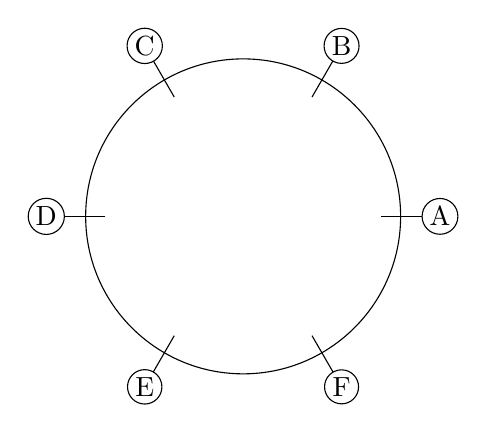
\begin{tikzpicture}
    \draw (0,0) circle (2);
    \draw (0:1.75) -- (0:2.5) node [draw, shape=circle, inner sep=1, fill=white, text=black] {A};
    \draw (60:1.75) -- (60:2.5) node [draw, shape=circle, inner sep=1, fill=white, text=black] {B};
    \draw (120:1.75) -- (120:2.5) node [draw, shape=circle, inner sep=1, fill=white, text=black] {C};
    \draw (180:1.75) -- (180:2.5) node [draw, shape=circle, inner sep=1, fill=white, text=black] {D};
    \draw (240:1.75) -- (240:2.5) node [draw, shape=circle, inner sep=1, fill=white, text=black] {E};
    \draw (300:1.75) -- (300:2.5) node [draw, shape=circle, inner sep=1, fill=white, text=black] {F};
\end{tikzpicture}

    \caption{Visualization of Ring Consistent Hashing}
    \label{fig:ring-hash-process}
\end{figure}
%
\begin{figure}
    \centering
    \begin{tikzpicture}
    \node (C) [draw, shape=circle, inner sep=1, fill=blue, text=white]
        at (0,0) {\(C\)};

    \node (B) [draw, shape=circle, inner sep=1, fill=white, text=black]
        at (-2,-2) {\(B\)};

    \node (E) [draw, shape=circle, inner sep=1, fill=white, text=black]
        at (2,-2) {\(E\)};

    \node (F) [draw, shape=circle, inner sep=1, fill=white, text=black]
        at (-3,-3) {\(F\)};

    \node (D) [draw, shape=circle, inner sep=1, fill=red, text=white]
        at (1,-3) {\(D\)};

    \node (A) [draw, shape=circle, inner sep=1, fill=white, text=black]
        at (3,-3) {\(A\)};

    \node (V) [draw, shape=diamond, inner sep=1, fill=orange, text=black]
        at (0,2) {\(v_n\)};

    \draw (F) to (B) to (C) to (E) to (A);
    \draw (D) to (E);

    \node at (2, 1.5) [text=orange] {\(\func{\procedure{Tree-Succ}}{tree, \func{h}{v_n}}\)};
    \draw [->, orange, thick] (V) to (C);
    \draw [->>, orange, thick] (C) to [out=180, in=90] (B);
    \draw [->>>, orange, thick] (B) to [out=0, in=-90] (C);

    \node at (3, 0) [text=blue] {\(\func{\procedure{Tree-Succ}}{tree, \func{h}{C.id}}\)};
    \draw [->, blue, thick, dotted] (C) to [out=0, in=90] (E);
    \draw [->>, blue, thick, dotted] (E) to [out=180, in=90] (D);
\end{tikzpicture}

    \caption{Red-Black Tree Traversal}
    \label{fig:tree-traversal}
\end{figure}
%
\begin{algorithm}
    \begin{algorithmic}
        \Procedure{Consistent-Hash}{$tree, key$}
            \State $p \gets \Call{Tree-Succ}{tree, \func{h}{key}}$
            \State $b \gets \Call{Tree-Succ}{tree, \func{h}{p.id}}$
            \State \Return $(p, b)$
        \EndProcedure
    \end{algorithmic}
    \caption{Consistent Hashing}
    \label{alg:consistent-hashing}
\end{algorithm}
%
\begin{algorithm}
    \begin{algorithmic}
        \Procedure{Tree-Succ}{$tree, key$}
            \If{$\func{h}{key} \geq \func{h}{\Call{Tree-Max}{tree}.id}$}
                \State \Return \Call{Tree-Min}{$tree$}
            \Else
                \State $root \gets \Call{Root}{tree}$
                \State \Return \Call{Recur-Succ}{$tree, root, root, key$}
            \EndIf
        \EndProcedure
    \end{algorithmic}
    \caption{Successor Node}
    \label{alg:tree-succ}
\end{algorithm}
%
\begin{algorithm}
    \begin{algorithmic}
        \Procedure{Recur-Succ}{$tree, root, succ, key$}
            \If{$root = null$}
                \State \Return $succ$
            \ElsIf{$key = \func{h}{root.id}$}
                \State $succ \gets \Call{Right}{root}$
                \If{$succ = null$}
                    \State $succ \gets root$
                    \While{$\Call{Par}{succ} \neq null \land \func{h}{succ} < key$}
                        \State $succ \gets \Call{Par}{succ}$
                    \EndWhile
                \Else
                    \While{$\Call{Left}{succ} \neq null$}
                        \State $succ \gets \Call{Left}{succ}$
                    \EndWhile
                \EndIf
                \Return {$succ$}
            \ElsIf{$\func{h}{root.id} > key$}
                \State $left \gets \Call{Left}{root}$
                \State \Return \Call{Recur-Succ}{$tree, left, root, key$}
            \Else
                \State $right \gets \Call{Right}{root}$
                \State \Return \Call{Recur-Succ}{$tree, right, succ, key$}
            \EndIf
        \EndProcedure
    \end{algorithmic}
    \caption{Recursively Determined Successor Node}
    \label{alg:recur-succ}
\end{algorithm}
%
\subsection{Consistency}
After we had decided on a method for determining \emph{where} to store data,
we needed a method of ensuring that the data actually arrived at the
appropriate node. To do this, we used the Two-Phase Commit protocol (2PC) which
ensures data consistency. It does this by checking that both slaves are
available: if so, the data is sent to both, if either is unavailable, the
unavailable node is handled and the process is restarted. \cite{tanenbaum2017}
%
\subsection{Fault Tolerance}
The primary reason for using consistent hashing is for fault tolerance. While
waiting for messages from the DBMS, the master pings each slave to ensure that
each slave node is still online. If it does not hear back from a slave after a
reasonable length of time (one second in our system), it assumes that the slave
is out of commission, and reallocates the vectors using \procedure{Reallocate}
(Algorithm~\ref{alg:reallocate}). In each node in the tree we store the
identifiers of the vectors on its associated slave, specifically for this
purpose.
\par
An example of this procedure can be seen in Figure~\ref{alg:reallocate}. There,
node \(F\) has failed, and the master had determined that vectors must be
reallocated. The vectors that must be reallocated are those for which \(F\) was
the primary location and those for which \(F\) was the backup location. First,
vectors \(v_1\) and \(v_2\) had \(F\) as their primary location and \(B\) as
their backup location (which will now become their primary location). So, \(B\)
will send (in one message) copies of \(v_1\) and \(v_2\) to node \(C\) which
will serve as the new backup location. Second, vectors \(v_4\) and \(v_5\) will
be sent (in one message) from \(A\) (their primary location) to \(B\) which
will take over as backup for \(F\). After this, the system will once again
contain two copies of each vector.
\par
%
In our implementation we utilized algorithms provided by \cite{cormen2009}
to find the predecessor of a slave (\procedure{Tree-Pred}), to find the
successor of a slave (\procedure{Tree-Succ}), and to delete a slave from the
tree (\procedure{RB-Delete}). We also made use of an RPC,
\(\func{\procedure{Send-Vector}}{s_1, k, s_2}\),
that we wrote which makes slave \(s_1\) send the vector \(k\) to slave \(s_2\).
\par
Using consistent hashing, we know that the failed slave's backup vectors are
the primary vectors of its predecessor. The successor must now maintain copies
of the predecessor's vectors, so the master notifies the predecessor to
communicate its primary vectors to the successor. Likewise, since the successor
node now holds the slave's primary vectors alongside its own, it must send the
slave's primary vectors to its successor as a backup.
\par
Consistent hashing is preferable to using a hash-mod-n technique, an algorithm
whose hash function modulus is the number of nodes. When the system changes
while using the hash-mod-n technique, it is possible that every single vector
would have to be remapped. This remapping requires significantly more message
passing than are used in the \procedure{Reallocate} function. This is because,
when a slave node is removed while using the hash-mod-n technique, the primary
locations of potentially every vector changes, thus requiring us to remap every
single vector in the worst case. \cite{kleppman2017} While hash-mod-n requires
\(\func{O}{K}\) remappings, where \(K\) is the number of keys, consistent
hashing only requires \(\func{O}{K/n}\) remappings where \(n\) is the number of
slaves. \cite{karger1997}
%
\begin{figure}
    \centering
    \begin{tikzpicture}
    \draw (0,0) circle (2);

    \node (A)
        [draw, shape=circle, inner sep=1, fill=white, text=black]
        at (95:2.5) {\(A\)};
    \node (A-in) at (95:1.75) {};
    \node (B)
        [draw, shape=circle, inner sep=1, fill=white, text=black]
        at (15:2.5) {\(B\)};
    \node (B-in)
        [draw, shape=circle, inner sep=1, color=white, fill=white, text=black]
        at (15:1.5) {\(M_1\)};
    \node (C)
        [draw, shape=circle, inner sep=1, fill=white, text=black]
        at (-70:2.5) {\(C\)};
    \node (C-in)
        [draw, shape=circle, inner sep=1, color=white, fill=white, text=black]
        at (-70:1.5) {\(M_2\)};
    \node (D)
        [draw, shape=circle, inner sep=1, fill=white, text=black]
        at (-150:2.5) {\(D\)};
    \node (D-in) at (-150:1.75) {};
    \node (E)
        [draw, shape=circle, inner sep=1, fill=white, text=black]
        at (-200:2.5) {\(E\)};
    \node (E-in) at (-200:1.75) {};
    \node (F)
        [draw, star, star points=13, star point ratio=2,
            inner sep=1, fill=red, text=black]
        at (60:2.5) {\(F\)};
    \node (F-in) at (60:1.75) {};

    \draw (A) -- (A-in);
    \draw (B) -- (B-in);
    \draw (C) -- (C-in);
    \draw (D) -- (D-in);
    \draw (E) -- (E-in);
    \draw (F) -- (F-in);


    \node (1)
        [draw, fill=orange, diamond, scale=0.5, label=above:{\(v_1\)}]
        at (70:2) {};
    \node (2)
        [draw, fill=orange, diamond, scale=0.5, label=above:{\(v_2\)}]
        at (85:2) {};
    \node (3)
        [draw, fill=orange, diamond, scale=0.5, label=above:{\(v_3\)}]
        at (30:2) {};
    \node (4)
        [draw, fill=orange, diamond, scale=0.5, label=above:{\(v_4\)}]
        at (110:2) {};
    \node (5)
        [draw, fill=orange, diamond, scale=0.5, label=above:{\(v_5\)}]
        at (130:2) {};

    \draw [->, thick, dashed] (1) -- (C-in);
    \draw [->, thick, dashed] (2) -- (C-in);

    \draw [->, thick, dotted] (4) -- (B-in);
    \draw [->, thick, dotted] (5) -- (B-in);
\end{tikzpicture}

    \caption{Visualization of Vector Reallocation}
    \label{fig:vector-reallocation}
\end{figure}
%
\begin{algorithm}
    \begin{algorithmic}
        \Procedure{Reallocate}{$tree, slave$}
            \State $pred \gets \Call{Tree-Pred}{tree, slave}$
            \State $succ \gets \Call{Tree-Succ}{tree, slave}$
            \State $ssucc \gets \Call{Tree-Succ}{tree, succ}$
            \ForAll{$v \in (slave.vectors \cap succ.vectors)$}
                \State \Call{Send-Vector}{$succ, v, ssucc$}
            \EndFor
            \ForAll{$w \in (slave.vectors \cap pred.vectors)$}
                \State \Call{Send-Vector}{$pred, w, succ$}
            \EndFor
            \State \Call{RB-Delete}{$tree, slave$}
        \EndProcedure
    \end{algorithmic}
    \caption{Reallocation}
    \label{alg:reallocate}
\end{algorithm}
%
\subsection{Queries}
Our system is designed to handle \term{range queries}. In this context, a range
query is a query written as a number of ranges which are \code{AND}ed together.
Each range is given as a pair of vector identifiers specifying the first and
last vector in a range. Within these ranges, the vectors are \code{OR}ed
together. An example of a range query is \code{R:[0,3]\&[5,7]} which would
correspond to a SQL query of the form
\code{SELECT * FROM . WHERE AGE~>~50 AND SALARY~>~\$100000}.
To carry out the query, we first create a plan that tells us which slave nodes
to visit.
%
\subsection{Query Planning}
Our query planning algorithm (Algorithm~\ref{alg:query-planning}) takes two
inputs. The first input, \(tree\), is the red-black tree used in consistent
hashing to determine which two nodes contain a given vector identifier.
The second input,
\[R = [\tuple{v_0, v_1}, \tuple{v_1, v_2}, \ldots, \tuple{v_n, v_m}],\]
is a list of tuples where each tuple denotes the first and last vectors of a
range. Each \(v_k\) is a vector identifier where \(0 \leq k \leq m\). Given the
tuple \(\tuple{v_i, v_j} \in R\), we require that
\(0 \leq i \leq j \leq n \leq m\). Sorting is performed so that, in each
portion of the query, slaves do not have to be visited more than once, making
query processing linear with respect to the number of slave nodes. Because
\(\lor\) is commutative, the order in which the vectors are \code{OR}ed
together within the subquery does not matter. Each range of the query may be
run concurrently. In an effort to distribute the work to all slaves as evenly
as possible, we choose a random return value from \procedure{Consistent-Hash}
as the slave to visit for each of the given vectors.
\par
The return value is a set \(Q\) of \term{subqueries}, where each subquery
comprises one or more tuples of the form \(\tuple{node\_id,vector\_id}\),
which will be used in the query execution algorithms to determine which slaves
to visit and which vectors to obtain.
%
\begin{algorithm}
    \begin{algorithmic}
        \Procedure{Range-Query-Plan}{$tree, R$}
            \State $swap \gets false$
            \State $paths \gets \emptyset$
            \ForAll{$r \in R$}
                \State $subpaths \gets \emptyset$
                \For{$k \gets r_0, r_1$}
                    \State $nodes \gets \Call{Consistent-Hash}{tree, k}$
                    \State $tuple \gets \emptyset$
                    \If{$swap$}
                        \State $tuple \gets tuple \cup \set{nodes_0}$
                    \Else
                        \State $tuple \gets tuple \cup \set{nodes_1}$
                    \EndIf
                    \State $tuple \gets tuple \cup \set{k}$
                    \State $subpaths \gets subpaths \cup tuple$
                \EndFor
                \State Sort $subpaths$ on $node.id$
                \State $paths \gets paths \cup subpath$
                \State $swap \gets \neg swap$
            \EndFor
            \Return $paths$
        \EndProcedure
    \end{algorithmic}
    \caption{Query Planning}
    \label{alg:query-planning}
\end{algorithm}
%
\subsection{Query Execution}
Execution of queries received by the master is handled using
Algorithm~\ref{alg:master-query-root} which first plans out the query using
Algorithm~\ref{alg:query-planning} and then delegates each subquery to its
slaves using Algorithm~\ref{alg:slave-subquery}.
\par
Algorithm~\ref{alg:slave-subquery} is an RPC that takes a node identifier,
denoting the slave that the function is run on, and a set of pairs, \(\gamma\),
representing a subquery. The slave iterates over the tuples referencing vectors
it contains, and \code{OR}s them together using WAH, as denoted by \(\lor\).
\(\func{\procedure{Retrieve-Vector}}{k}\) returns the value of vector \(k\).
Once the slave has operated on all requested vectors it holds, it makes an RPC
to the slave in the subsequent tuple, recursively satisfying the remainder of
the subquery.
\par
Algorithm~\ref{alg:master-query-root} takes a complete query, divides the work
among the slaves, \code{AND}s the results of the subqueries (denoted by
\(\lambda\)) together, and returns the result to the DBMS.
%
\begin{algorithm}
    \begin{algorithmic}
        \Procedure{Master-Query-Root}{$Q$}
            \State $R \gets \emptyset$
            \ForAll{$subquery \in Q$}
                \Comment{Delegate subqueries.}
                \State $slave\_id \gets subquery[0][0]$
                \State $r \gets \Call{Range-SubQuery}{slave\_id, subquery}$
                \State $R \gets R \cup \set{r}$
            \EndFor
            \State $v \gets \vec{1}$
            \ForAll{$w \in R$}
                \Comment{\code{AND} the results.}
                \State $v \gets v \land w$
            \EndFor
            \State \Return $v$
        \EndProcedure
    \end{algorithmic}
    \caption{Master Query Root}
    \label{alg:master-query-root}
\end{algorithm}
%
\begin{algorithm}
    \begin{algorithmic}
        \Procedure{Range-SubQuery}{$node\_id,q$}
            \State $r \gets \vec{0}$
            \ForAll{$tuple \in q$}
                \If{$tuple_0 = node\_idd$}
                    \State $r \gets r \lor \Call{Retrieve-Vector}{tuple_1}$
                    \State $q \gets q \setminus \set{tuple}$
                \Else
                    \State $s \gets \Call{Range-SubQuery}{tuple_0, q}$
                    \State $r \gets r \lor s$
                \EndIf
            \EndFor
            \State \Return $r$
        \EndProcedure
    \end{algorithmic}
    \caption{Slave subquery}
    \label{alg:slave-subquery}
\end{algorithm}
%
\subsection{Implementation and Testing Notes}
Due to its speed and established usage in systems like ours, such as Redis
\cite{redis}, we settled on writing our system primarily in the C programming
language. In addition to C, Python~3 was used to script the production of
testing data, which we obtained from the TPC-C data repository. Python~3 was
also used in collaboration with bash to produce startup scripts that
facilitated automatic testing of the system. In order to create our RPCs, we
had to specify the types of RPCs being used in the ONC+ RPC language which is
an extension of the eXternal Data Representation (XDR) language developed in
the mid 1980s by Sun Microsystems.
